\section{WEB SCRAPING}
\subsection{Giới thiệu Web scraping}
\begin{enumerate}
    \item []
    \hspace*{0.7cm} Web Scraping \cite{noauthor_web_2024} là một phương pháp trích xuất dữ liệu từ các trang web bằng phần mềm tự động lưu thông tin ở định dạng có tổ chức.\\
    
    \hspace*{0.7cm}Thay vì sao chép và dán thủ công từng phần thông tin như cách truyền thống, phương pháp này cho phép chúng ta thu thập dữ liệu với số lượng lớn trong thời gian ngắn. Đặc biệt, với nhu cầu phân tích và xử lý dữ liệu ngày càng tăng, web scraping trở thành công cụ hữu ích để trích xuất thông tin từ nhiều nguồn khác nhau trên internet mà không cần tốn quá nhiều công sức.
\end{enumerate}

\subsection{Nguyên lý hoạt động}
\begin{enumerate}
    \item []
    \hspace*{0.7cm}Quy trình hoạt động của web scraping gồm các bước:
    
    \begin{figure}[h]
        \centering
        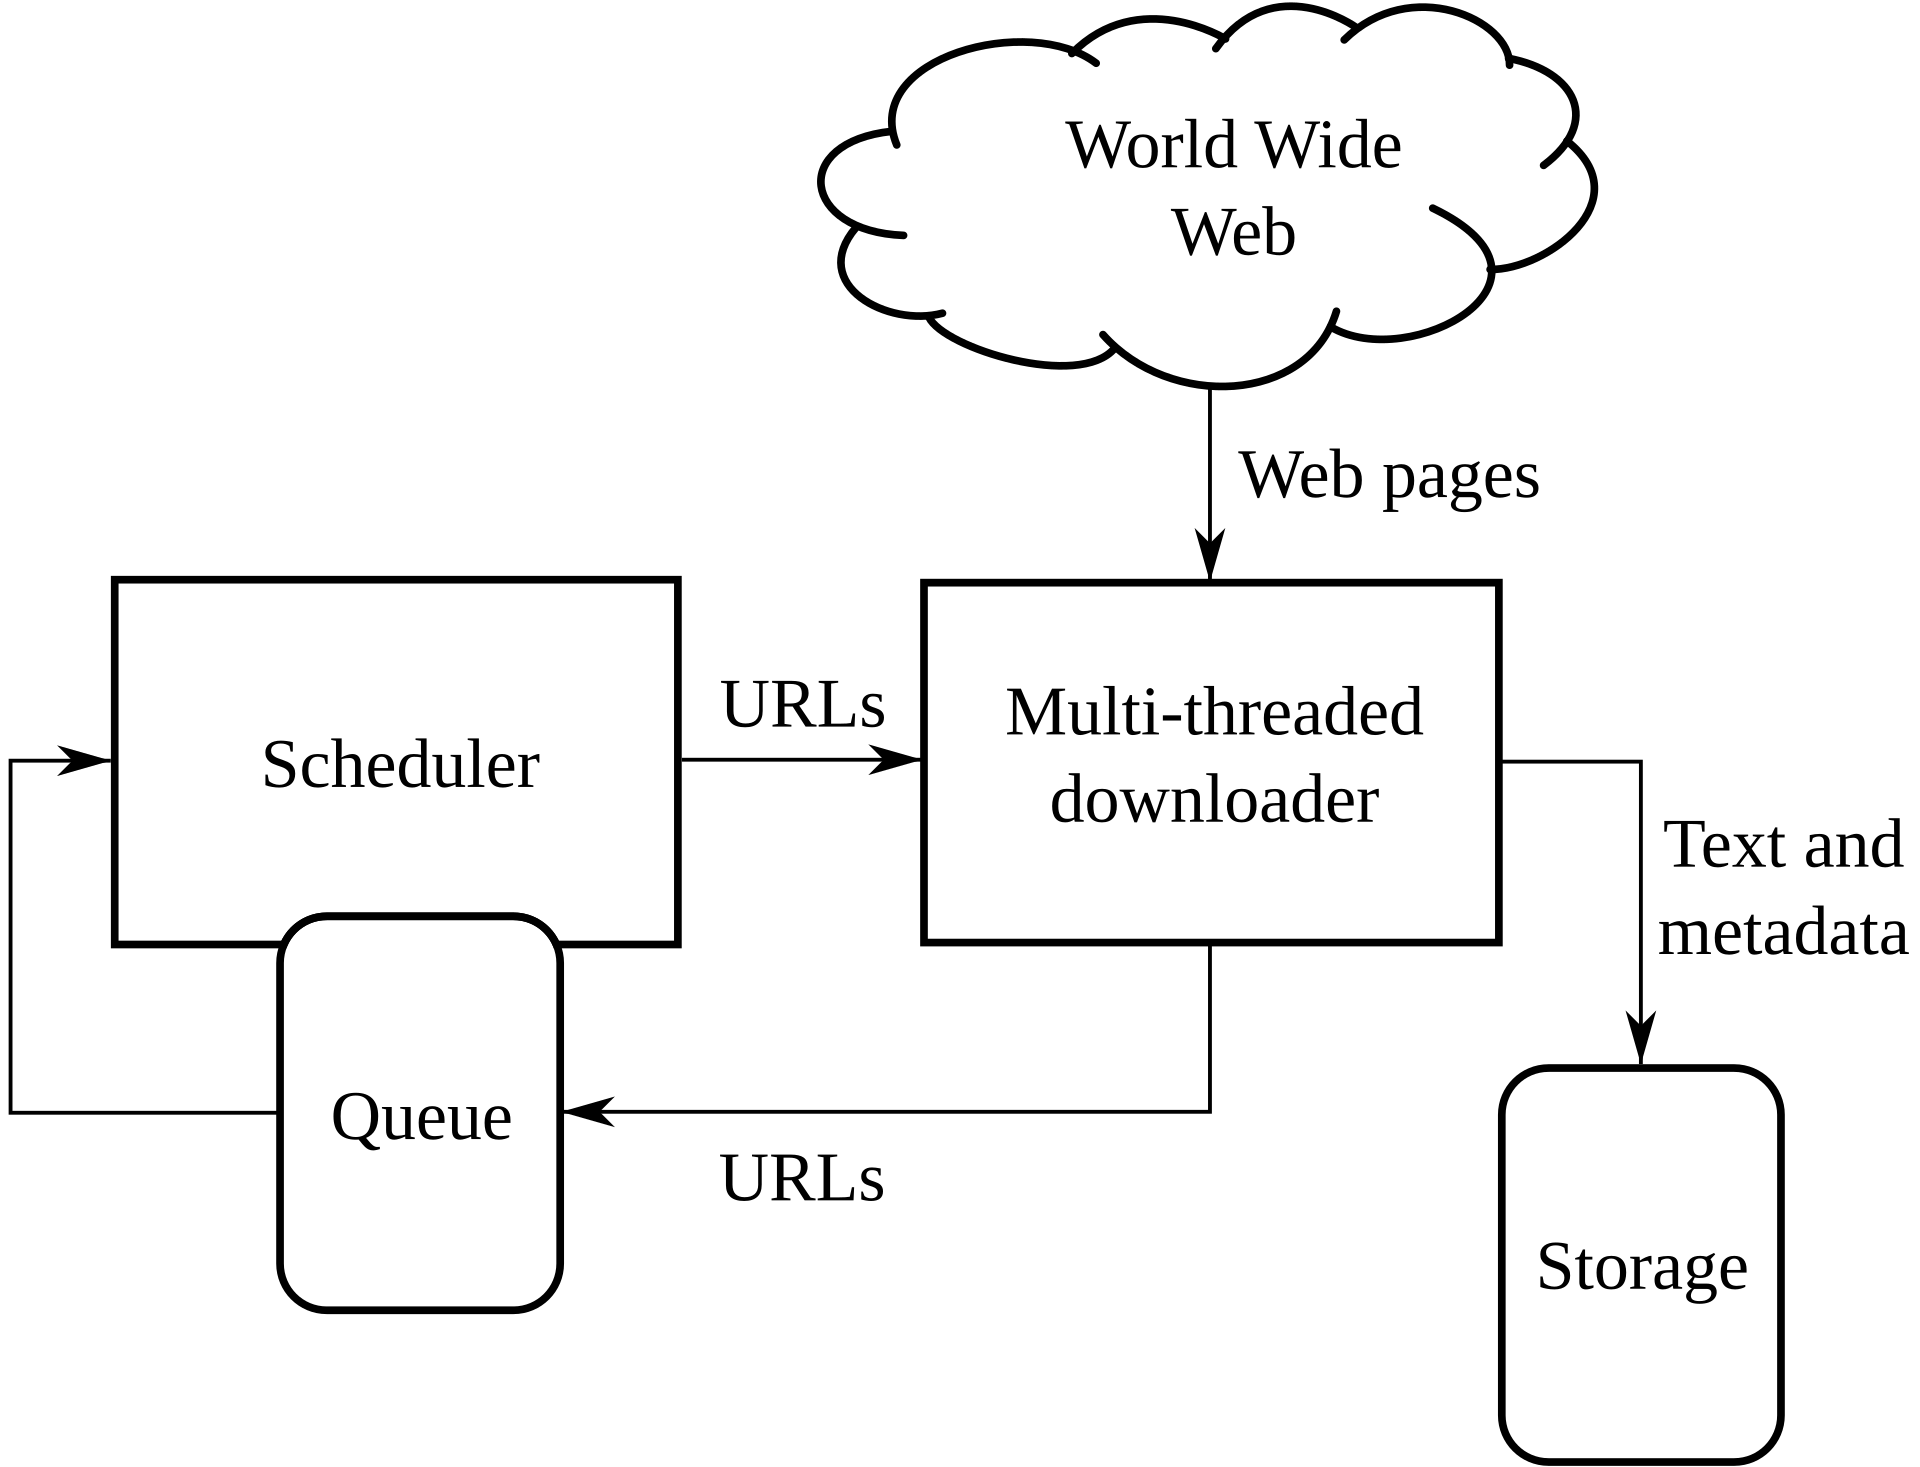
\includegraphics[width=0.6\linewidth]{img/img_chuong2/WebCrawler.svg.png}
        \caption{Quy trình Web scarping. Nguồn \cite{noauthor_1920px-webcrawlerarchitecturesvgpng_nodate} }
        \label{fig:web_scraping}
    \end{figure}
    
    \begin{itemize}[left=0.7cm] 
        \item[-]\textbf{Xác định website mục tiêu}: Đây là trang web mà bạn muốn thu thập dữ liệu từ đó.
        
        \item[-]\textbf{Thu thập URL}: Lấy địa chỉ URL của website mà bạn muốn trích xuất thông tin.
        
        \item[-]\textbf{Gửi yêu cầu}: Tạo yêu cầu HTTP để lấy HTML của website mục tiêu.
        
        \item[-] \textbf{Tìm dữ liệu}: Sử dụng bộ định vị để xác định vị trí dữ liệu trong HTML.
        
        \item[-] \textbf{Lưu dữ liệu}: Ghi lại dữ liệu đã trích xuất vào file JSON, CSV hoặc các định dạng cấu trúc khác.
        

        
    \end{itemize}
  
    
    
\end{enumerate}

\subsection{Ưu điểm và hạn chế}
\begin{enumerate}
    \item []
    \textbf{Ưu điểm:}
    \begin{itemize}[left=0.5cm] 
    \item[-] \textbf{Tự động hóa quy trình thu thập dữ liệu}: Web scraping cho phép giảm thiểu thời gian và công sức so với phương pháp thu thập dữ liệu truyền thống.
    
    \item[-] \textbf{Khả năng thu thập dữ liệu quy mô lớn}: Người dùng có thể lấy thông tin từ nhiều trang web khác nhau chỉ trong một khoảng thời gian ngắn.
    
    \item[-] \textbf{Cập nhật dữ liệu liên tục}: Các công cụ web scraping có thể được cấu hình để tự động làm mới dữ liệu theo thời gian thực, đảm bảo thông tin luôn chính xác và cập nhật.
    
    \item[-] \textbf{Hỗ trợ phân tích thông tin}: Cung cấp dữ liệu hữu ích cho việc đánh giá và nghiên cứu các lĩnh vực khác nhau.
    
    \item[-] \textbf{Theo dõi biến động thông tin}: Giúp giám sát sự thay đổi của các yếu tố liên quan một cách hiệu quả.
    \end{itemize}
\end{enumerate}

\begin{enumerate}
    \item []
    \textbf{Hạn chế:}
    \begin{itemize}[left=0.5cm] 
        \item[-] \textbf{Vấn đề pháp lý}: Việc thu thập dữ liệu từ các trang web có thể dẫn đến vi phạm điều khoản dịch vụ, gây ra rủi ro pháp lý cho người thực hiện.
        
        \item[-] \textbf{Khó khăn với trang web động}: Các trang web sử dụng JavaScript hoặc công nghệ tải động có thể làm khó khăn trong quá trình thu thập dữ liệu.
        \newpage
        
        \item[-] \textbf{Yêu cầu kiến thức kỹ thuật}: Để thực hiện web scraping hiệu quả, người dùng cần nắm vững lập trình, cấu trúc HTML và các giao thức web.
        
        \item[-] \textbf{Đạo đức và trách nhiệm}: Quy trình thu thập và tổ chức thông tin từ các trang web có thể gây ra những lo ngại về tính hợp pháp và công bằng trong việc sử dụng dữ liệu. Do đó, người dùng cần thực hiện web scraping một cách có trách nhiệm, tôn trọng quyền riêng tư và tuân thủ các quy định của trang web để bảo vệ quyền lợi của các bên liên quan.\cite{noauthor_web_2021}

        
    \end{itemize}
\end{enumerate}